\documentclass{scrartcl}
\usepackage[utf8]{inputenc}
\usepackage{ngerman}
\usepackage{tikz}
\usetikzlibrary{arrows,decorations.pathmorphing,backgrounds,fit,positioning,shapes.symbols,chains,shapes.geometric,shapes.arrows,calc}

\begin{document}
  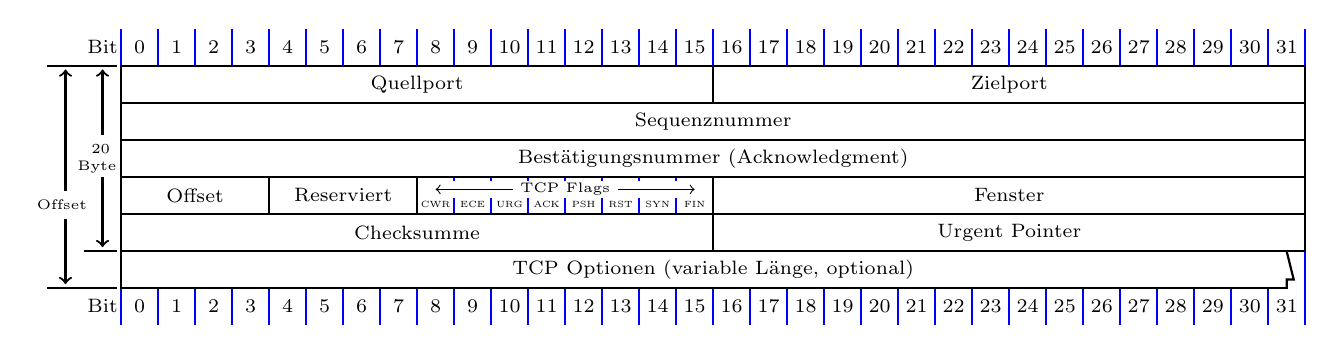
\begin{tikzpicture}[scale=0.47]
	\foreach \x in {0,...,31}
		\node at (\x+0.5,20.5) {\scriptsize \x};
	\foreach \x in {0,...,31}
		\node at (\x+0.5,13.5) {\scriptsize \x};
	\foreach \x in {0,...,32}
		\draw[thick, blue] (\x,13) -- (\x,21);
	\node[thick] (bit1) at (-0.5,20.5) {\scriptsize Bit};
	\node[thick] (bit2) at (-0.5,13.5) {\scriptsize Bit};
	\draw [<->, thick] (-0.5, 19.9) -- (-0.5,15.1);
	\draw [<->, thick] (-1.5, 19.9) -- (-1.5,14.1);
	\draw [thick] (-2, 20) -- (-0.1,20);
	\draw [thick] (-1, 15) -- (-0.1,15);
	\draw [thick] (-2, 14) -- (-0.1,14);
	\filldraw[white] (-1.45,18) rectangle (-0.1,17);
	\node[fill=white] at (-0.55,17.75) {\tiny 20};
	\node at (-0.65,17.25) {\tiny Byte};
	\node[fill=white] at (-1.6,16.25) {\tiny Offset};
	\filldraw[thick,draw=black, fill=white] (0,20) rectangle (16,19); \node (mode) at (8,19.5) {\scriptsize Quellport};
	\draw[thick, draw=black, fill=white] (16,20) rectangle (32,19); \node (li) at (24,19.5) {\scriptsize Zielport};
	\filldraw[thick,draw=black, fill=white] (0,19) rectangle (32,18); \node (mode) at (16,18.5) {\scriptsize Sequenznummer};
	\filldraw[thick,draw=black, fill=white] (0,18) rectangle (32,17); \node (mode) at (16,17.5) {\scriptsize Best\"atigungsnummer (Acknowledgment)};
	\draw[thick, draw=black, fill=white] (0,17) rectangle (4,16); \node (li) at (2,16.5) {\scriptsize Offset};
	\draw[thick, draw=black, fill=white] (4,17) rectangle (8,16); \node (li) at (6,16.5) {\scriptsize Reserviert};
	\draw[thick, draw=black] (8,17) rectangle (16,16);\filldraw[white] (8.5,16.43) rectangle (15.8,16.88);\draw[<->] (8.5,16.66) -- (15.5,16.66); 
	\filldraw[white] (10.6,16.43) rectangle (13.4,16.88); \node at (12,16.66) {\tiny TCP Flags};
	\node[scale=0.65] at (8.5,16.25) {\tiny CWR};
	\node[scale=0.65] at (9.5,16.25) {\tiny ECE};
	\node[scale=0.65] at (10.5,16.25) {\tiny URG};
	\node[scale=0.65] at (11.5,16.25) {\tiny ACK};
	\node[scale=0.65] at (12.5,16.25) {\tiny PSH};
	\node[scale=0.65] at (13.5,16.25) {\tiny RST};
	\node[scale=0.65] at (14.5,16.25) {\tiny SYN};
	\node[scale=0.65] at (15.5,16.25) {\tiny FIN};
	\draw[thick, draw=black, fill=white] (16,17) rectangle (32,16); \node (li) at (24,16.5) {\scriptsize Fenster};
	\filldraw[thick,draw=black, fill=white] (0,16) rectangle (16,15); \node (mode) at (8,15.5) {\scriptsize Checksumme};
	\filldraw[thick, draw=black, fill=white] (16,16) rectangle (32,15); \node (li) at (24,15.5) {\scriptsize Urgent Pointer};
	\draw[thick,draw=black, fill=white] (0,15) rectangle (31.5,14);
	\draw[fill=white, draw=white] (31.4,14.96) rectangle (31.6,14.05);
	\draw[thick]  (31.5,14.97)  decorate [decoration=saw] { -- (31.5,14.02)};
	\node (mode) at (16,14.5) {\scriptsize TCP Optionen (variable L\"ange, optional)};
    \end{tikzpicture}
  \end{document}
